\documentclass[a4paper]{article}
\usepackage{subfigure}
\usepackage{amsmath,amssymb,algorithmic,booktabs,bm,caption,cases,csvsimple,enumerate,float,geometry,graphicx,indentfirst,listings,makecell,multirow,setspace,tabularx,titlesec,xcolor}
\geometry{left=3.5cm,right=3.5cm,top=3.3cm,bottom=3.3cm}
\lstset{
	language=Matlab, numbers=left, tabsize=4,
	framexleftmargin=1.5mm, frame=leftline,
	keywordstyle=\color{blue}\bfseries,
	identifierstyle=\bf, breaklines=true, 
	basicstyle=\normalsize,rulecolor=\color{brown}, 
	numberstyle=\color[RGB]{20,20,20}
}
\begin{document}
\begin{titlepage}
	\begin{Large}
		\begin{center}
			\noindent\rule[0.25\baselineskip]{\textwidth}{1pt}
			\vspace{0.5cm}
			\textsc{UM--SJTU Joint Institute}\\
			\vspace{0.25cm}
			\textsc{Signals and Systems\\(VE216)}
			\noindent\rule[0.25\baselineskip]{\textwidth}{1pt}
			\vspace{4.9cm}\\
			\textsc{Laboratory Report}\\
			\vspace{0.85cm}
			\textsc{Lab 3}\\
			\vspace{0.5em}
			Feedback Control
			\vspace{6cm}
		\end{center}
	\end{Large}
	\begin{tabular}{ll}
		Name: Yihua Liu&ID:518021910998\\
		&\\
		Date: \today&\\
	\end{tabular}
\end{titlepage}
\newpage
\renewcommand\thesection{\arabic{section}}
\section{Objectives}
\begin{itemize}
    \item Understand feedback control.
\end{itemize}
\section{Theoretical Background}
\subsection{A Closed-Loop Feedback Model}
The block diagram of a generic closed-loop feedback control system is shown in Figure 1. In this figure, the "plant" is the system whose output we wish to control. A measurement is performed on the output by the measurement sub-system, which is then compared with the desired output, i.e., the input to the control system. The output of the comparator, which computes the difference between the desired and the actual output, is fed into a controller whose output servers as the input to the plant. If the comparator and measurement system were removed from the above diagram then one would be left with an open-loop (i.e., no feedback) controller.
\begin{figure}[H]
    \begin{center}
        \includegraphics[width=0.8\textwidth]{1.png}
    \end{center}
    \caption{Closed-Loop Control System. The plant is the generic term for the system to be controlled.}
\end{figure}
\subsection{Closed-Loop Transfer Function}
As mentioned earlier, we will restrict our discussion to the case where all of the blocks shown in Figure 1 are LTI systems. Thus the input/output relationship of each of these blocks can be described by a system transfer function. Furthermore, we will realize the comparator as an adder and change the gain on the measurement to -1. With these changes, the block diagram of Figure 2 becomes:
\begin{figure}[H]
    \begin{center}
        \includegraphics[width=0.8\textwidth]{2.png}
    \end{center}
    \caption{Closed-Loop Feedback Control System. (C: Controller, P: Plant, M: Measurement)}
\end{figure}
It is a simple matter of algebra to compute the closed-loop transfer function, $G_{cl}(s)=Y(s)/X(s)$, of the system shown in Figure 1 as indicated below.
\begin{equation}
    Y(s)=E(s)C(s)P(s)
\end{equation}
\begin{equation}
    E(s)=X(s)-H(s)Y(s)
\end{equation}
Combining Eqs. (1) and (2) yields
\begin{equation}
    G_{cl}(s)=\frac{Y(s)}{X(s)}=\frac{C(s)P(s)}{1+C(s)P(s)H(s)}
\end{equation}
\begin{equation}
    \frac{E(s)}{X(s)}=\frac{1}{1+C(s)P(s)H(s)}
\end{equation}
\subsection{Examples of Feedback Control Systems}
\subsubsection{DC Motor Model}
Let us assume that we want to control the shaft position of a DC motor. To help design a controller for this DC motor, we mathematically model the angular position, $\theta(t)$ of the shift by the following differential equation
\begin{equation}
    \frac{\mathrm{d}^2\theta(t)}{\mathrm{d}t^2}+\frac{\mathrm{d}\theta(t)}{\mathrm{d}t}=V(t)
\end{equation}
where $V(t)$ is the voltage applied to the motor. Thus the plant (i.e., the motor) is an LTI system that has the following system transfer function
\begin{equation}
    P(s)=\frac{1}{s(s+1)}
\end{equation}
This transfer function corresponds to a second-order LTI system with no zeros, and a pair of real poles located at the origin and at -1.
\subsubsection{No Controller}
Suppose we want the shaft of the motor to rotate by one radian per second by using a unit step as the input, i.e., $V(t)=u(t)$. Then
\begin{equation}
    \theta(s)=V(s)P(s)=\frac{1}{s}\frac{1}{s(s+1)}=-\frac{1}{s}+\frac{1}{s^2}+\frac{1}{s+1}
\end{equation}
where the right-most side of Eq. (7) is obtained by a partial fraction expansion. Consequently,
\begin{equation}
    \theta(t)=(t-1+e^{-t})u(t)
\end{equation}
which is clearly not going to achieve the desired rotation by one radian per second!
\subsubsection{Controller Without Feedback (i.e., Open-Loop Control)}
Shown below is the block diagram of an open-loop controller. We choose a differentiator as the controller,
\begin{figure}[H]
    \begin{center}
        \includegraphics[width=0.5\textwidth]{3.png}
    \end{center}
    \caption{Open-Loop Controller}
\end{figure}
i.e.,
\begin{equation}
    C(s)=s
\end{equation}
of a unit-step input. Thus
\begin{equation}
    \theta(s)=V(s)C(s)P(s)=\frac{1}{s}s\frac{1}{s(s+1)}=\frac{1}{s}-\frac{1}{s+1}
\end{equation}
Therefore
\begin{equation}
    \theta(t)=(1-e^{-t})u(t)
\end{equation}
Clearly, $\lim_{t\rightarrow\infty}\theta(t)=1$, so that this controller results in no steady-state error (i.e., $e(t)=V(t)-\theta(t)=0$ as $t\rightarrow\infty$ when the input is a unit step. The response of the DC motor to the unit step, however, is rather slow. It takes approximately 2.3 s for the shaft angle to reach 90\% of its final value of 1 radian.

We might ask how well this same controller would work if the input were a ramp rather than a step. Under such circumstances
\begin{equation}
    V(s)=\frac{1}{s^2}
\end{equation}
\begin{equation}
    \theta(s)=V(s)C(s)P(s)=\frac{1}{s^2}s\frac{1}{s(s+1)}=-\frac{1}{s}+\frac{1}{s^2}+\frac{1}{s+1}
\end{equation}
Therefore
\begin{equation}
    \theta(t)=(t-1+e^{-t})u(t)
\end{equation}
and the steady-state error is 1 radian/second. Thus the angular position of the shift deviates from the desired position by 1 radian as $t\rightarrow\infty$, and this differentiator-controller is inadequate for a ramp input.
\subsubsection{Sensitivity of an Open-Loop Controller to Plant Changes}
Suppose that overheating changes the transfer function of the motor by a small amount to become
\begin{equation}
    P(s)=\frac{1}{(s+0.01)(s+1)}
\end{equation}
i.e., one of the poles has moved along the real axis from the origin into the left-hand plane (LHP). The step response of the motor now becomes
\begin{equation}
    \theta(s)=V(s)C(s)P(s)=\frac{1}{s}s\frac{1}{(s+0.01)s(s+1)}=\frac{100/99}{s+0.01}-\frac{100/99}{s+1}
\end{equation}
Therefore
\begin{equation}
    \theta(t)=(100/99)(e^{-0.01t}-e^{-t})u(t)
\end{equation}
and in steady state $\lim_{t\rightarrow\infty}\theta(t)=0$, yielding a steady state error of one radian. It is clear that this open-loop controller is quite sensitive to variations in the plant transfer function.
\subsubsection{Feedback (or Closed-Loop) Control}
Consider now the feedback control system shown in Figure 2 with $H(s)=1$, $C(s)=Ks$ (i.e., a differential controller) and $P(s)=1/[s(s+1)]$ as before. Then according to Eq. (3) the closed-loop transfer function is given by
\begin{equation}
    G_{cl}(s)=\frac{Y(s)}{X(s)}=\frac{C(s)P(s)}{1+C(s)P(s)H(s)}=\frac{KsP(s)}{1+KsP(s)}=\frac{K}{s+(K+1)}
\end{equation}
and the step response becomes
\begin{equation}
    \theta(s)=V(s)G_{cl}(s)=\frac{1}{s}\frac{K}{s+(K+1)}=\frac{K/(K+1)}{s}-\frac{K/(K+1)}{s+(K+1)}
\end{equation}
or equivalently
\begin{equation}
    \theta(t)=\frac{K}{K+1}(1-e^{-(K+1)t})u(t).
\end{equation}
If $K$ is sufficiently large, then the steady-state error, $\lim_{t\rightarrow\infty}(V(t)-\theta(t))=1/(K+1)$ will be small. Also note that the response time is much improved over that obtained by an open-loop controller. In particular, the 90\% rise-time has been reduced from 2.3 s to $2.3/(K+1)$s.
\subsubsection{Sensitivity of the Closed-Loop Controller to Plant Changes}
As before we will consider the situation where the transfer function of the motor changes by a small amount to become that given by Eq. (15). Using the same feedback controller described above, the closed-loop response becomes
\begin{equation}
    G_{cl}(s)=\frac{Ks}{s^2+(1.01+K)s+0.01}.
\end{equation}
Thus the step response is given by
\begin{equation}
    \theta(s)=\frac{K}{s^2+(1.01+K)s+0.01}=\frac{K/(a_+-a_-)}{s+a_+}-\frac{K/(a_+-a_-)}{s+a_-}
\end{equation}
where
\begin{equation}
    a_\pm=\frac{(1.01+K)\mp\sqrt{(1.01+K)^2-0.04}}{2}.
\end{equation}
Therefore for $K$ large $a_+\approx0$ and $a_-\approx K$, yielding the step response
\begin{equation}
    \theta(t)\approx(1-e^{-Kt})u(t)
\end{equation}
Notice that with this closed-loop controller the step response is relatively insensitive to small changes in the plant.
\subsubsection{Using Feedback to Stabilize Unstable Systems}
Consider a plant that has the following transfer function
\begin{equation}
    P(s)=\frac{1}{s-1}
\end{equation}
This system is not bounded-input/bounded-output (BIBO) stable, since its transfer function has a pole in the right-half plane. It is easy to verify, for example, that the unit step response of this system is given by $(-1+e^t)u(t)$ and hence is not bounded. By implementing the feedback system shown in Figure 2 with $H(s)=1$ and $C(s)=K$, the closed-loop transfer function becomes
\begin{equation}
    G_{cl}(s)=\frac{C(s)P(s)}{1+C(s)P(s)}=\frac{1}{s+(K-1)}
\end{equation}
Thus for $K>1$, the pole has been moved into the LHP and the system has become BIBO stable.
\section{Experiment Procedures}
\subsection{Open Loop Control--Plant}
\begin{figure}[H]
    \begin{center}
        \includegraphics[width=0.5\textwidth]{4.jpg}
    \end{center}
    \caption{Plant Circuit}
\end{figure}
Steps:
\begin{enumerate}
    \item Construct the plant circuit according to Figure 4. Where $R_0=10k\Omega$, $C_1=100\mu$F, $C_2=0.22\mu$F.
    \item Impulse response: A=1V, width=0.1s, f=1Hz. (1 Picture)
    \item Step Response: A=1V, f=1Hz. (1 Picture)
\end{enumerate}
For example, for the step response, you should try to get something like the waveform shown in following figure.
\begin{figure}[H]
    \begin{center}
        \includegraphics[width=0.5\textwidth]{5.jpg}
    \end{center}
    \caption{Plant Result}
\end{figure}
\textbf{Note 1: Do not destroy your plant circuit after you get the image, you are going to use it in the next part.}

\textbf{Note 2: Do not forget to supply all the op-amps with DC voltage(Pin 4(-12V) and 7(12V))}

\textbf{Note 3: If a capacitor is labeled"474", its capacitance is $47\times10^4$pF; "224" is $22\times10^4$pF}
\begin{figure}[H]
    \begin{center}
        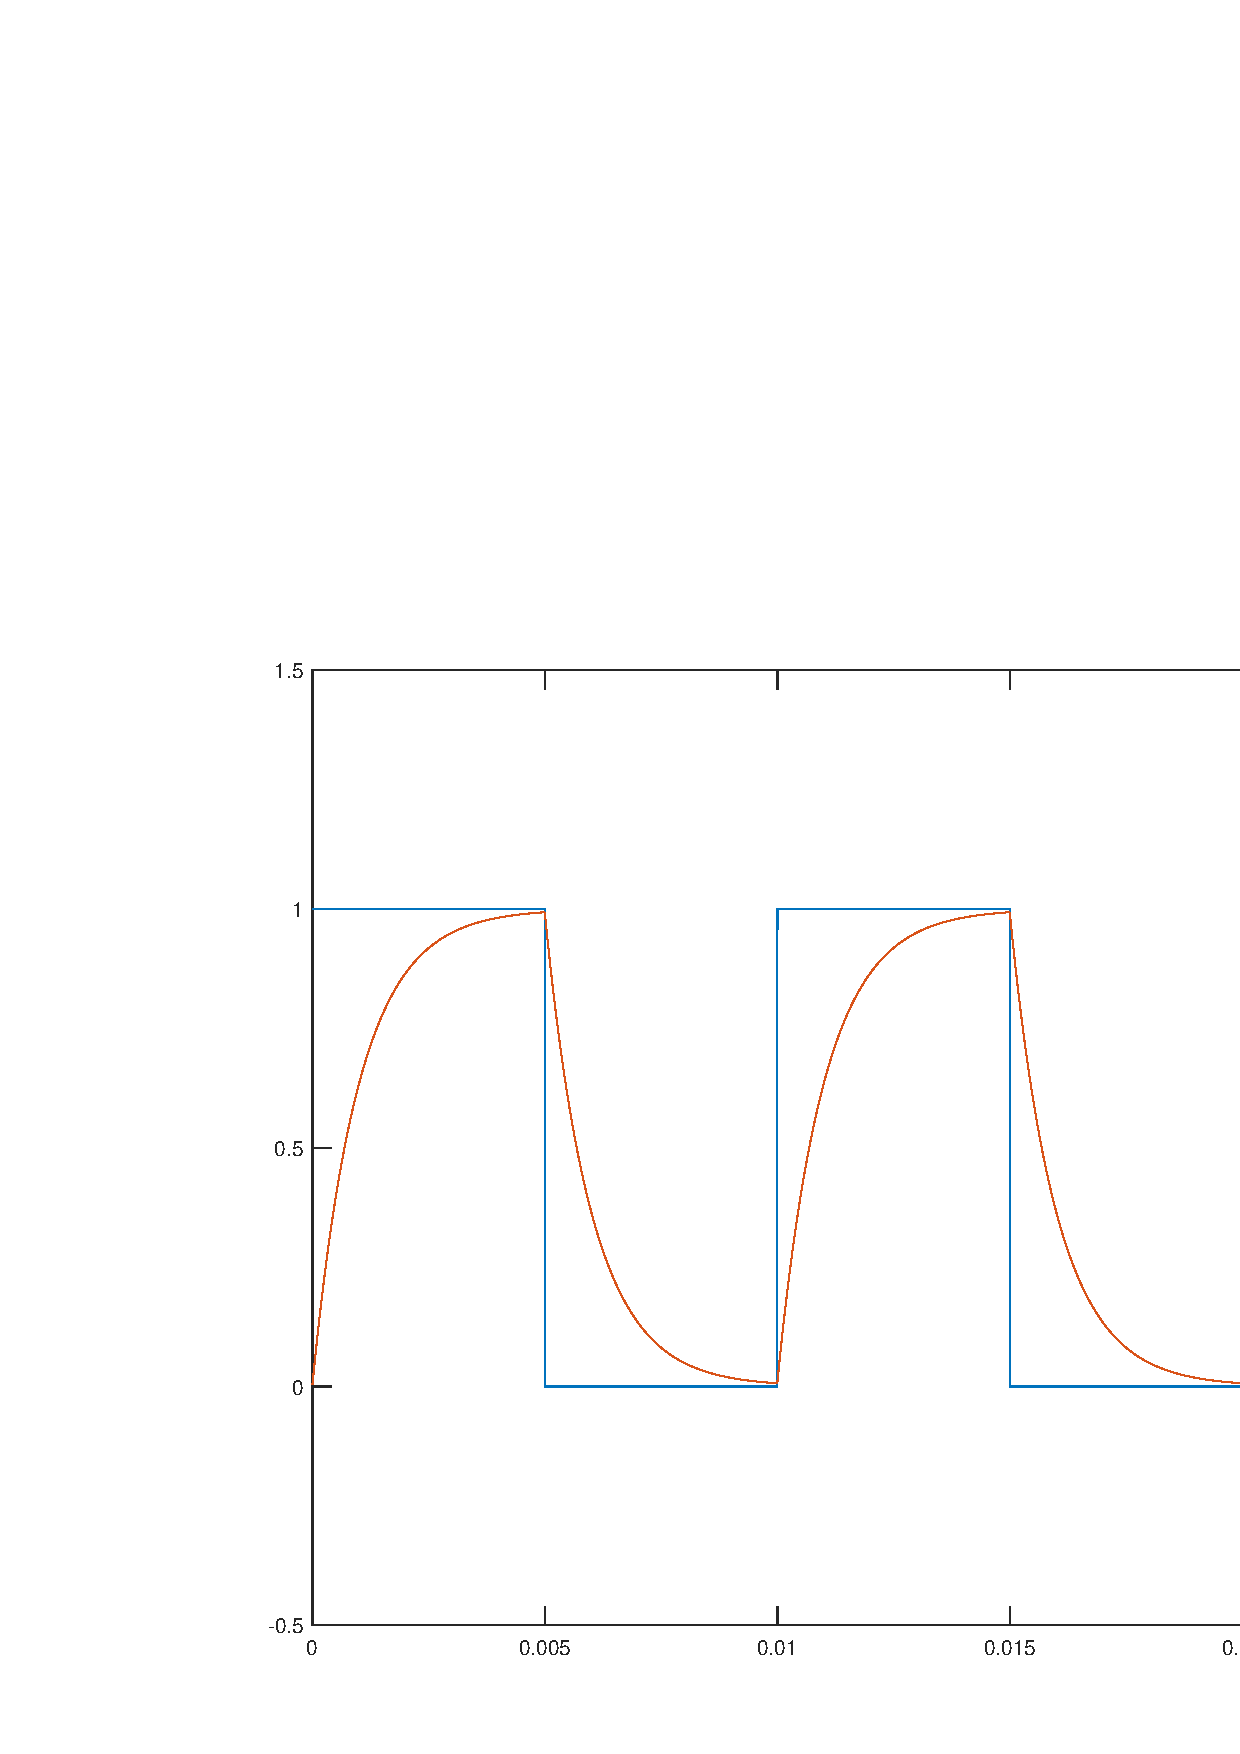
\includegraphics[width=0.4\textwidth]{6.jpg}
    \end{center}
    \caption{Op-amp}
\end{figure}
\subsection{Feedback Control}
\begin{figure}[H]
    \begin{center}
        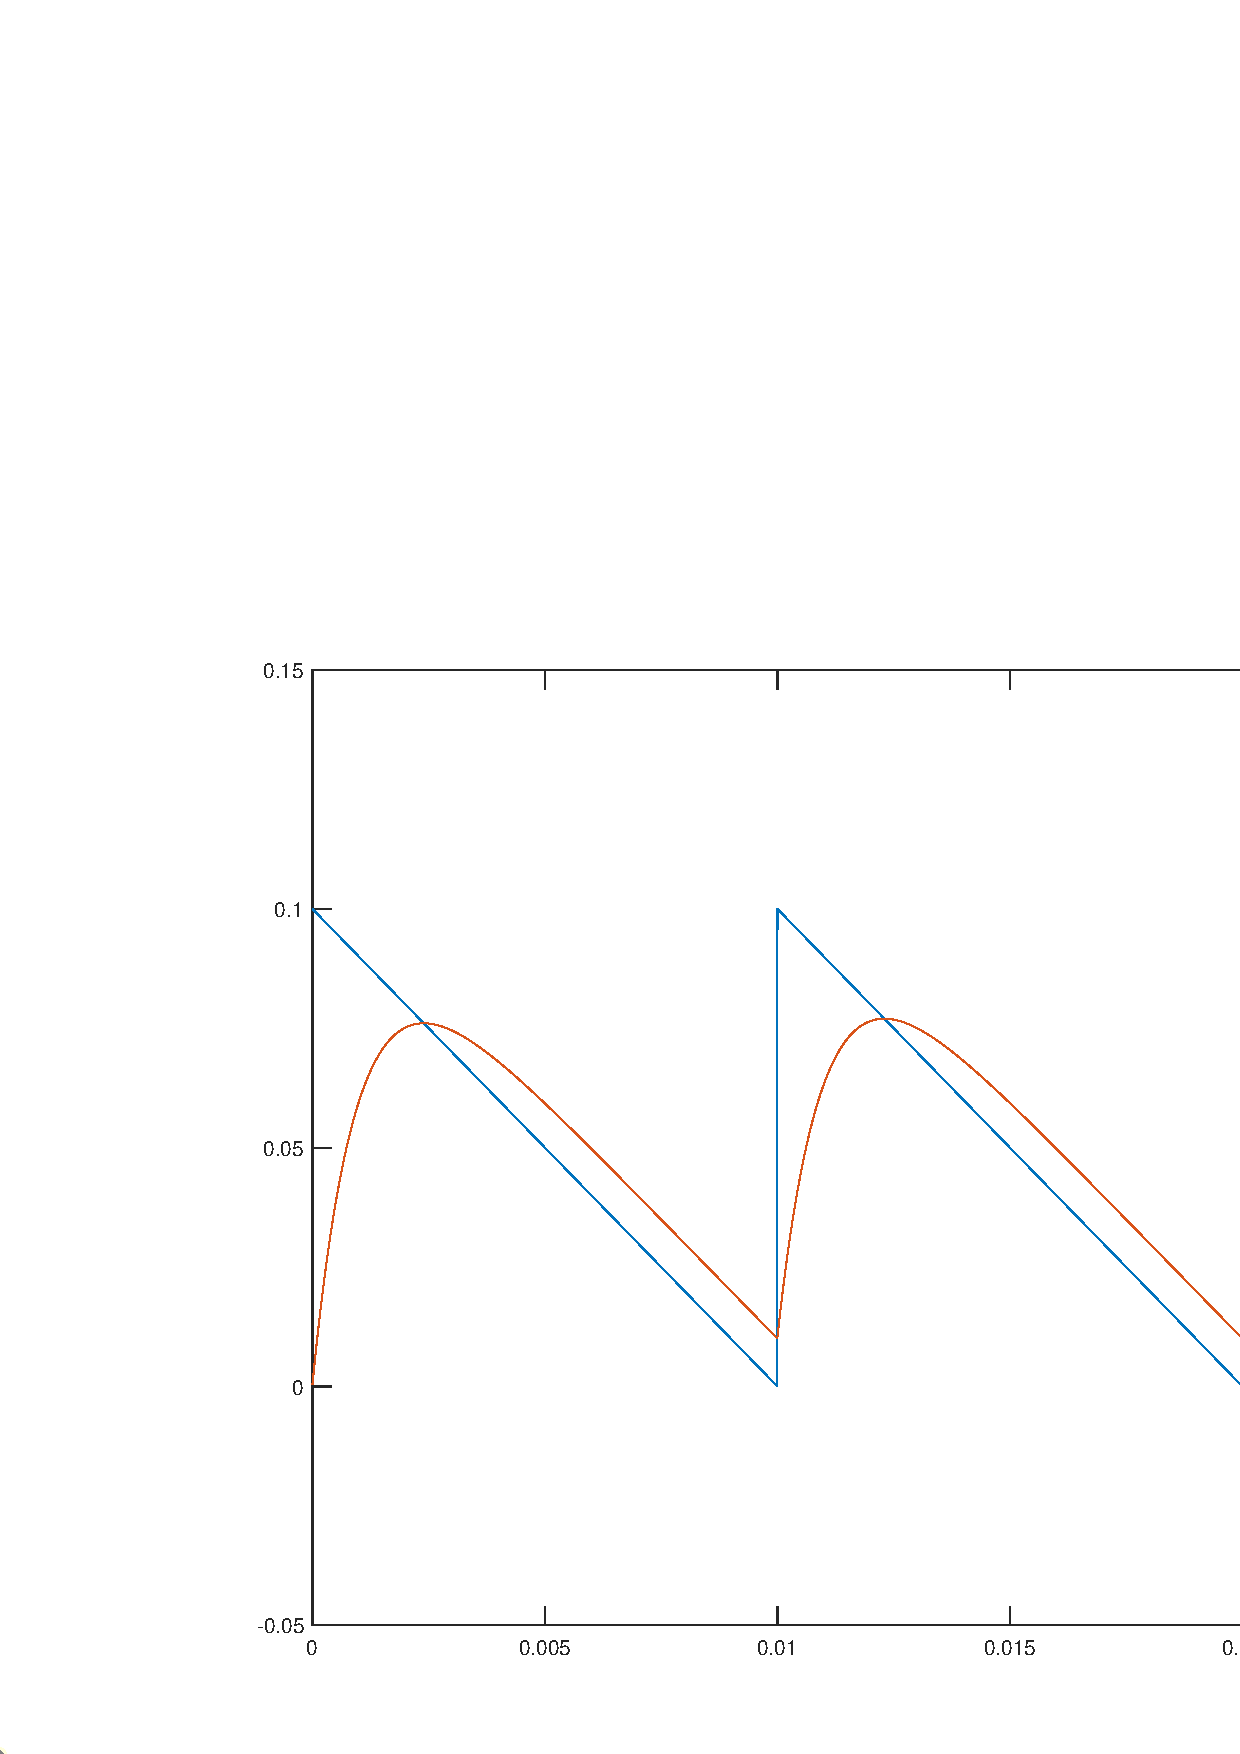
\includegraphics[width=0.5\textwidth]{7.jpg}
    \end{center}
    \caption{Feedback Control Circuit}
\end{figure}
Steps:
\begin{enumerate}
    \item Add the feedback control circuit to the plant according to Figure 7. Where $R_1=R_3=150k\Omega$, $R_2=3k\Omega$, $C_3=0.47\mu$F.
    \item Impulse response: A=1V, width=0.1s, f=1Hz. (1 Picture)
    \item Step Response: A=1V, f=1Hz. (1 Picture)
\end{enumerate}
For example, for step response, you should try to get something like the waveform shown in the following figure.
\begin{figure}[H]
    \begin{center}
        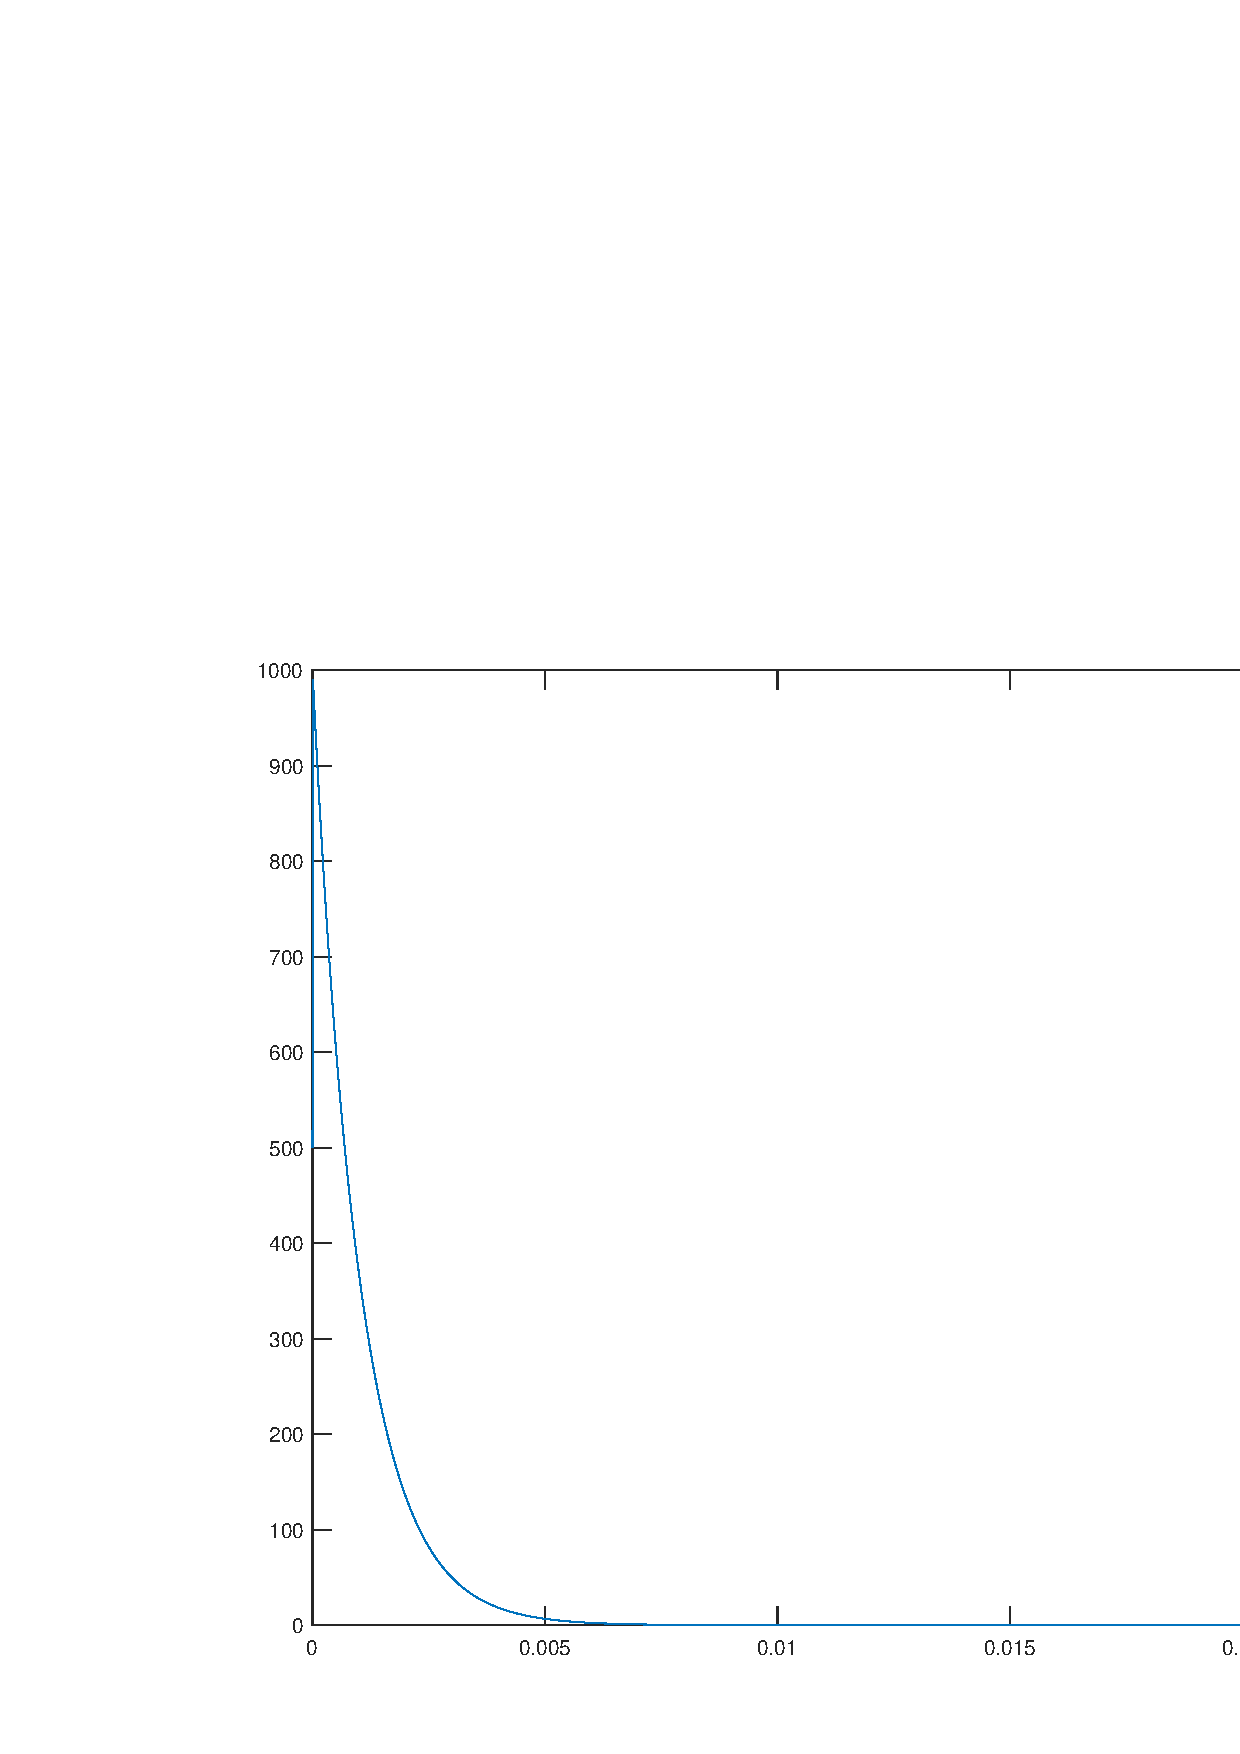
\includegraphics[width=0.6\textwidth]{8.jpg}
    \end{center}
    \caption{Feedback Control Result}
\end{figure}
\section{Experimental Results}
\subsection{Open Loop Control--Plant}
For impulse response: A=1V, width=0.1s, f=1Hz:
\begin{figure}[H]
    \begin{center}
        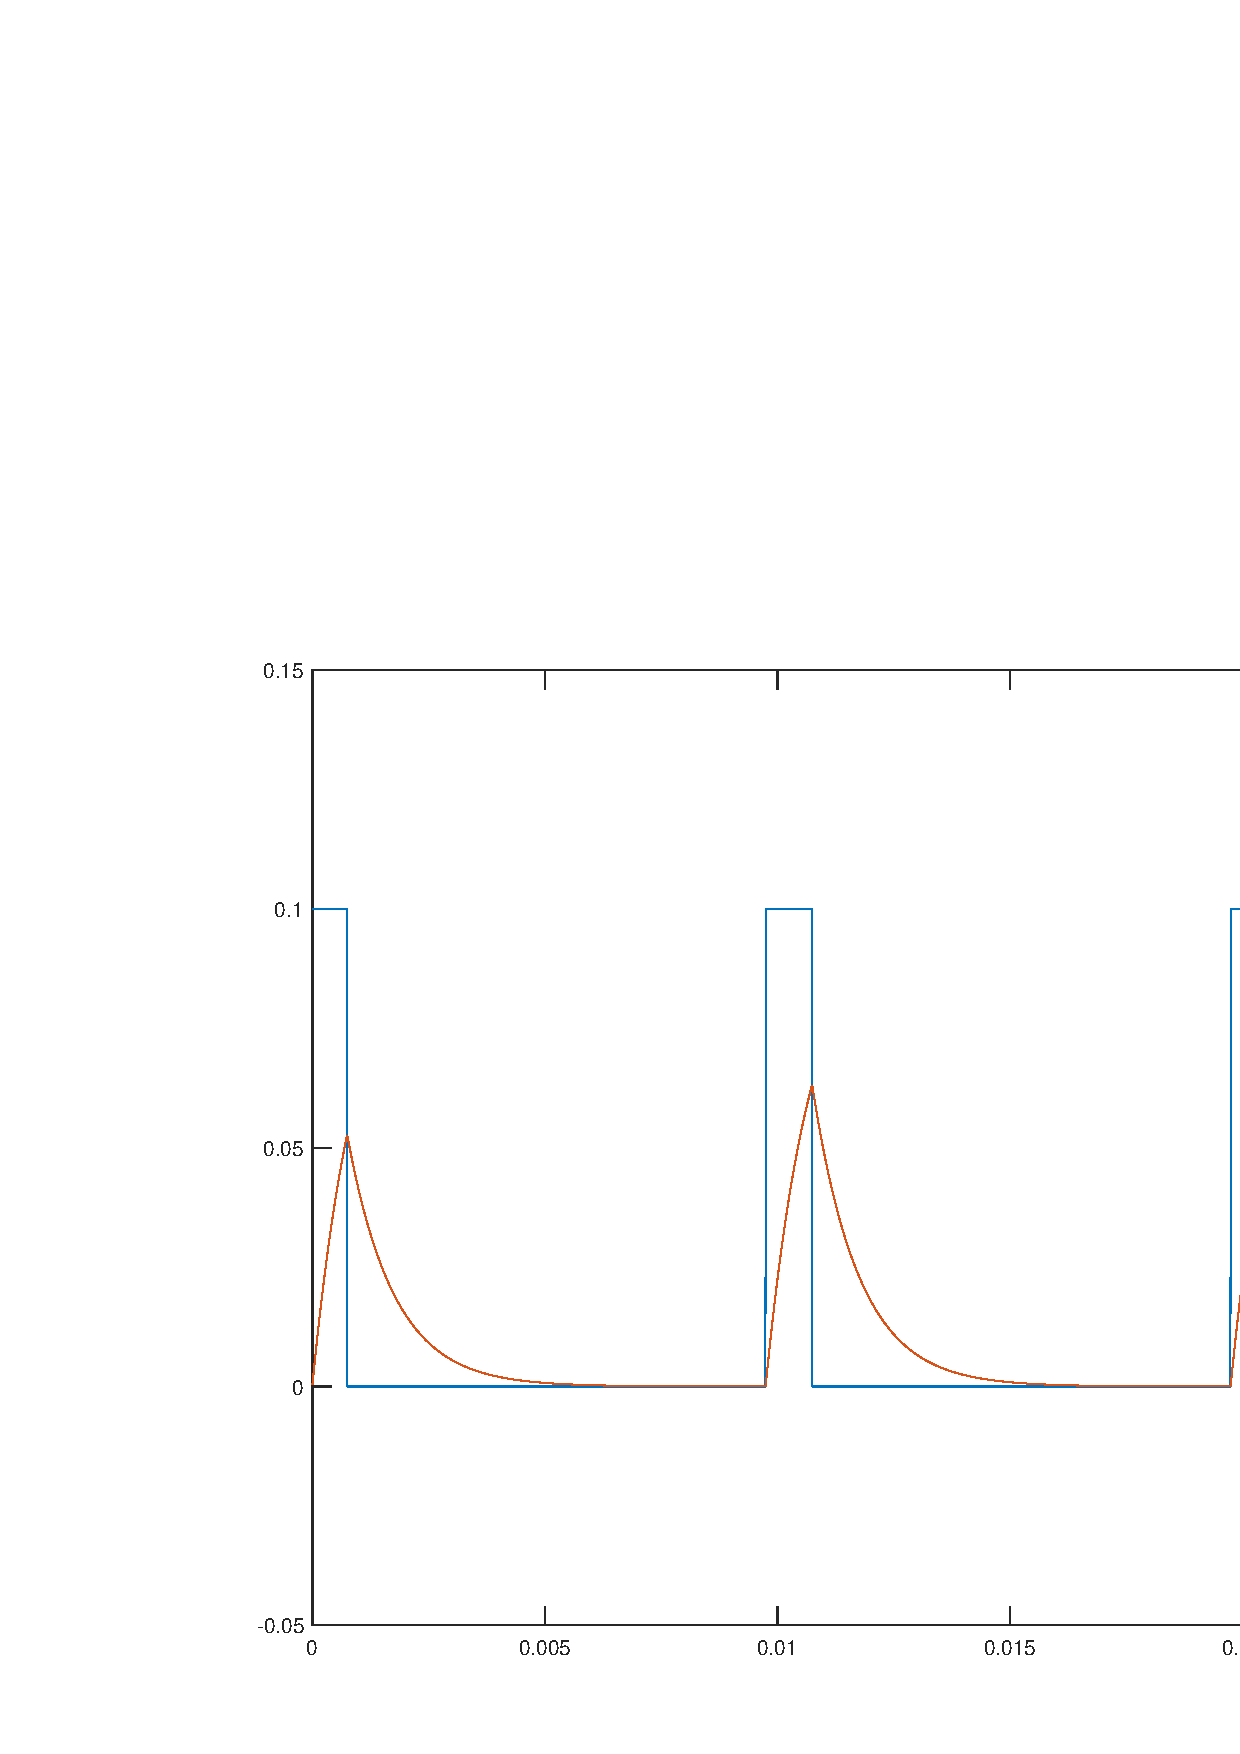
\includegraphics[width=0.8\textwidth]{9.png}
    \end{center}
    \caption{Impulse response for open loop control--plant: A=1V, width=0.1s, f=1Hz.}
\end{figure}
For step Response: A=1V, f=1Hz:
\begin{figure}[H]
    \begin{center}
        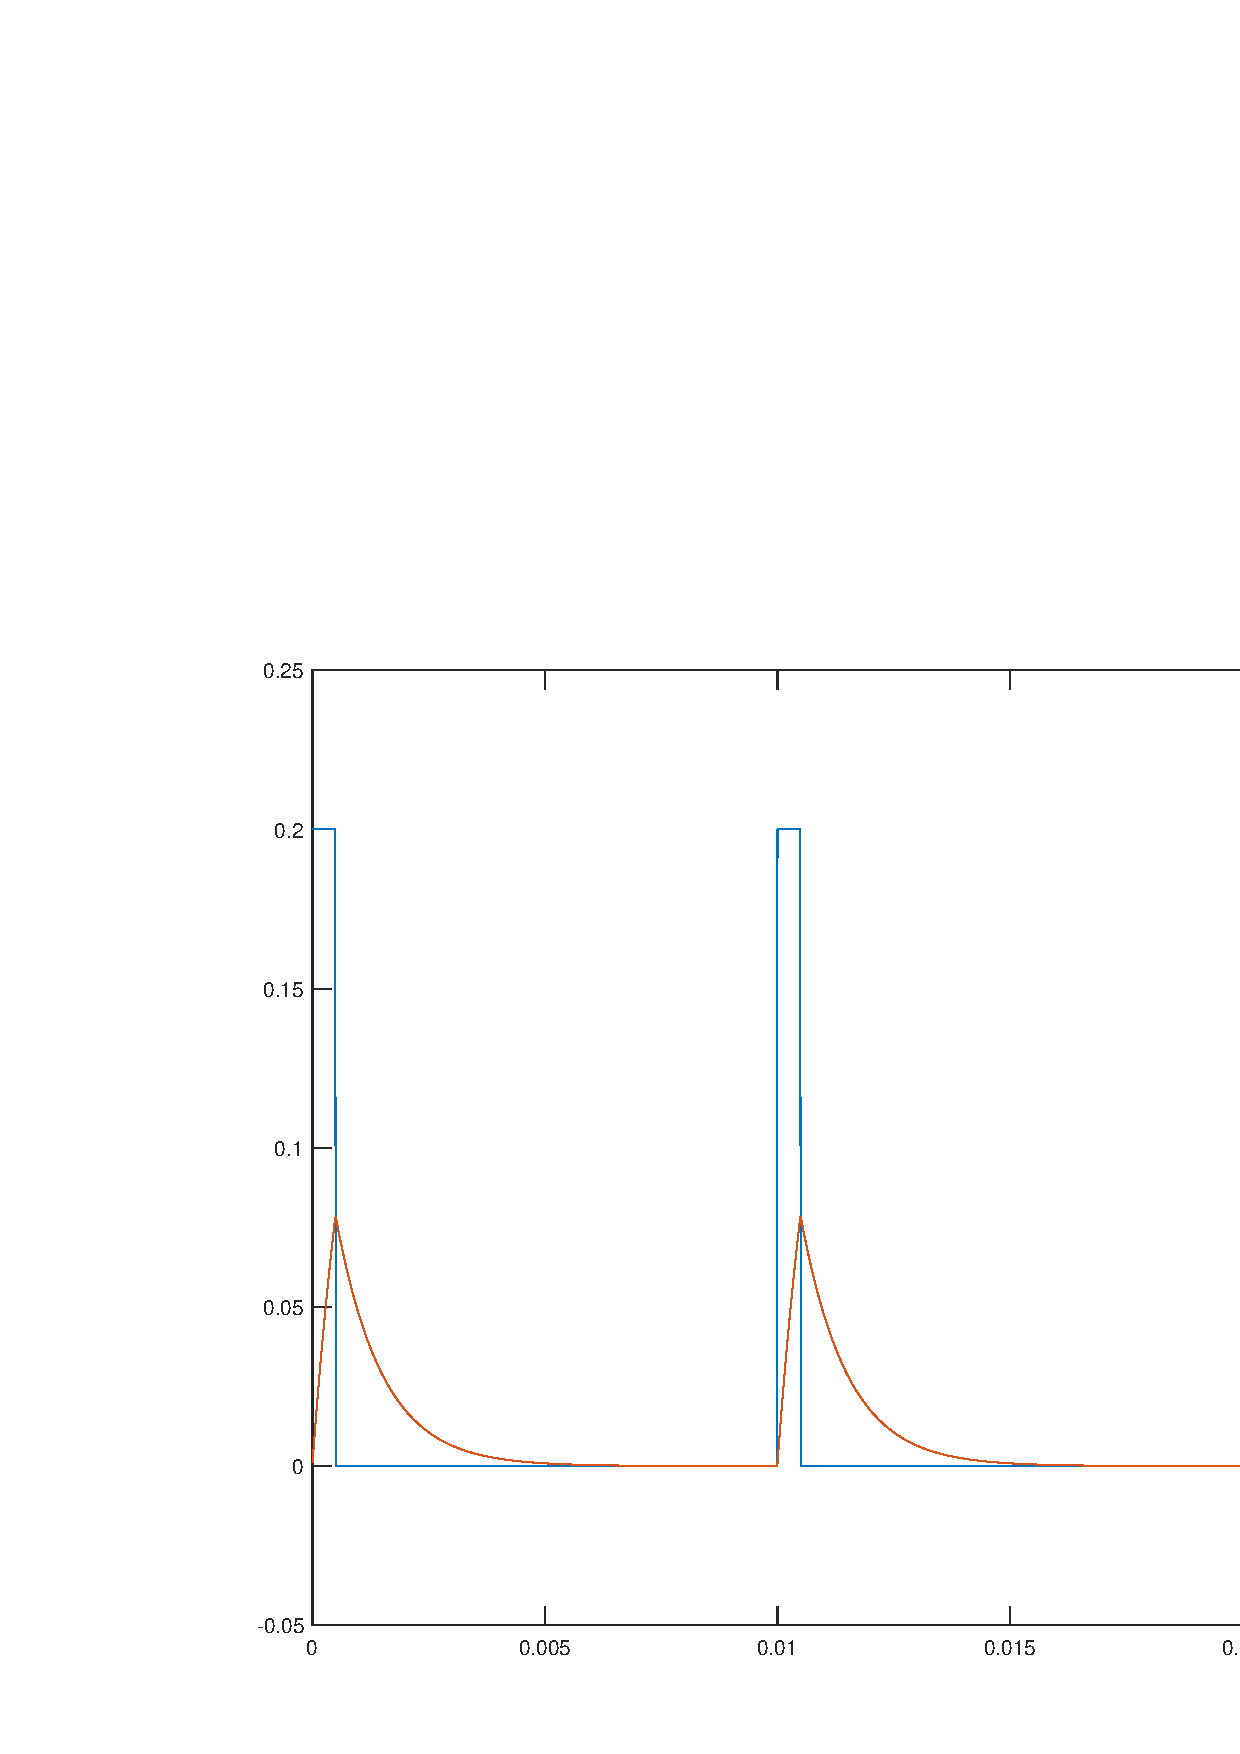
\includegraphics[width=0.8\textwidth]{10.png}
    \end{center}
    \caption{Step response for open loop control--plant: A=1V, f=1Hz.}
\end{figure}
\subsection{Feedback Control}
For impulse response: A=1V, width=0.1s, f=1Hz:
\begin{figure}[H]
    \begin{center}
        \includegraphics[width=0.8\textwidth]{11.png}
    \end{center}
    \caption{Impulse response for feedback control: A=1V, width=0.1s, f=1Hz.}
\end{figure}
For step Response: A=1V, f=1Hz:
\begin{figure}[H]
    \begin{center}
        \includegraphics[width=0.8\textwidth]{12.png}
    \end{center}
    \caption{Step response for feedback control: A=1V, f=1Hz.}
\end{figure}
\section{Error Analysis and Discussion}
In the experiment, the graphs for all the four cases meet our expectations. Since the traditional operational amplifier LM741 would fail in Proteus simulation with error "timestep too small" because it uses SPICE model and SPICE library, we use LF351 instead to simulate our circuits. The error may come from the internal design of the applied operational amplifier because they are real operational amplifiers rather than ideal ones.
\section{Conclusion}
In this lab, we successfully achieved our goals.

First, we understood the open loop control and feedback control. After the experiment, we analyzed the errors occurred during the experiment.

Second, we reviewed the closed-loop feedback model and its transfer function that we learned in VE216 lectures. Then, we extend to more feedback control systems and open-loop control systems using Laplace Transform and partial fraction expansion. Besides, we also analyzed their sensitivities and applications.

Finally, we got more familiar with operational amplifiers, signal generators and digital oscilloscopes.
\section{Reference}
\begin{enumerate}
	\item Lab 3: Feedback Control Part I: Intro \& Pre-lab Assignment Borrowed from UMich EECS 216.
	\item Lab3 Manual.
\end{enumerate}
\end{document}